
%%%%%%%%%%%%%%%%%%%%%%%%%%%%% Define Article %%%%%%%%%%%%%%%%%%%%%%%%%%%%%%%%%%
\documentclass[conference]{IEEEtran}
%%%%%%%%%%%%%%%%%%%%%%%%%%%%%%%%%%%%%%%%%%%%%%%%%%%%%%%%%%%%%%%%%%%%%%%%%%%%%%%

%%%%%%%%%%%%%%%%%%%%%%%%%%%%% Using Packages %%%%%%%%%%%%%%%%%%%%%%%%%%%%%%%%%%
\usepackage{geometry}
\usepackage{graphicx}
\usepackage{amssymb}
\usepackage{amsmath}
\usepackage{amsthm}
    
\usepackage{empheq}
\usepackage{mdframed}
\usepackage{booktabs}
\usepackage{lipsum}
\usepackage{graphicx}
\usepackage{color}
\usepackage{psfrag}
\usepackage{pgfplots}
\usepackage{bm}
\usepackage[spanish]{babel}
\usepackage[utf8]{inputenc} % Codificación UTF-8
\usepackage{amsmath}        % Soporte para ecuaciones matemáticas
\usepackage{graphicx}       % Manejo de imágenes
\usepackage{hyperref}       % Hipervínculos
\usepackage{caption}        % Formato para figuras
\usepackage{multirow}
\usepackage{subcaption}
\usepackage{biblatex}
\usepackage{csquotes}
\usepackage{bookmark}
%%%%%%%%%%%%%%%%%%%%%%%%%%%%%%%%%%%%%%%%%%%%%%%%%%%%%%%%%%%%%%%%%%%%%%%%%%%%%%%

% Other Settings

%%%%%%%%%%%%%%%%%%%%%%%%%% Page Setting %%%%%%%%%%%%%%%%%%%%%%%%%%%%%%%%%%%%%%%
\geometry{a4paper, margin=1in}

%%%%%%%%%%%%%%%%%%%%%%%%%% Define some useful colors %%%%%%%%%%%%%%%%%%%%%%%%%%
\definecolor{ocre}{RGB}{243,102,25}
\definecolor{mygray}{RGB}{243,243,244}
\definecolor{deepGreen}{RGB}{26,111,0}
\definecolor{shallowGreen}{RGB}{235,255,255}
\definecolor{deepBlue}{RGB}{61,124,222}
\definecolor{shallowBlue}{RGB}{235,249,255}
%%%%%%%%%%%%%%%%%%%%%%%%%%%%%%%%%%%%%%%%%%%%%%%%%%%%%%%%%%%%%%%%%%%%%%%%%%%%%%%

%%%%%%%%%%%%%%%%%%%%%%%%%% Define an orangebox command %%%%%%%%%%%%%%%%%%%%%%%%
\newcommand\orangebox[1]{\fcolorbox{ocre}{mygray}{\hspace{1em}#1\hspace{1em}}}
%%%%%%%%%%%%%%%%%%%%%%%%%%%%%%%%%%%%%%%%%%%%%%%%%%%%%%%%%%%%%%%%%%%%%%%%%%%%%%%

%%%%%%%%%%%%%%%%%%%%%%%%%%%% English Environments %%%%%%%%%%%%%%%%%%%%%%%%%%%%%
\newtheoremstyle{mytheoremstyle}{3pt}{3pt}{\normalfont}{0cm}{\rmfamily\bfseries}{}{1em}{{\color{black}\thmname{#1}~\thmnumber{#2}}\thmnote{\,--\,#3}}
\newtheoremstyle{myproblemstyle}{3pt}{3pt}{\normalfont}{0cm}{\rmfamily\bfseries}{}{1em}{{\color{black}\thmname{#1}~\thmnumber{#2}}\thmnote{\,--\,#3}}
\theoremstyle{mytheoremstyle}
\newmdtheoremenv[linewidth=1pt,backgroundcolor=shallowGreen,linecolor=deepGreen,leftmargin=0pt,innerleftmargin=20pt,innerrightmargin=20pt,]{theorem}{Theorem}[section]
\theoremstyle{mytheoremstyle}
\newmdtheoremenv[linewidth=1pt,backgroundcolor=shallowBlue,linecolor=deepBlue,leftmargin=0pt,innerleftmargin=20pt,innerrightmargin=20pt,]{definition}{Definition}[section]
\theoremstyle{myproblemstyle}
\newmdtheoremenv[linecolor=black,leftmargin=0pt,innerleftmargin=10pt,innerrightmargin=10pt,]{problem}{Problem}[section]
%%%%%%%%%%%%%%%%%%%%%%%%%%%%%%%%%%%%%%%%%%%%%%%%%%%%%%%%%%%%%%%%%%%%%%%%%%%%%%%

%%%%%%%%%%%%%%%%%%%%%%%%%%%%%%% Plotting Settings %%%%%%%%%%%%%%%%%%%%%%%%%%%%%
\usepgfplotslibrary{colorbrewer}
\pgfplotsset{width=8cm,compat=1.9}
%%%%%%%%%%%%%%%%%%%%%%%%%%%%%%%%%%%%%%%%%%%%%%%%%%%%%%%%%%%%%%%%%%%%%%%%%%%%%%%

%%%%%%%%%%%%%%%%%%%%%%%%%%%%%%% Title & Author %%%%%%%%%%%%%%%%%%%%%%%%%%%%%%%%
\author{\IEEEauthorblockN{Carlos Fernando Torres Ferrer, Daniel Fernando Aranda Contreras, Dairo Alexander Lobo Moreno,\\ Yulieth Valentina Portilla Jaimes}
\IEEEauthorblockA{Escuela E3T, Universidad Industrial de Santander\\
Correo electrónico: \{carlos2221116, daniel2221648, dairo2221123, yulieth2221136\}@correo.uis.edu.co}}
%%%%%%%%%%%%%%%%%%%%%%%%%%%%%%%%%%%%%%%%%%%%%%%%%%%%%%%%%%%%%%%%%%%%%%%%%%%%%%%
\begin{document}
% Título
\title{\uppercase{Diseño de infraestructura eléctrica de la nueva subestación Huila 230 kV y líneas de transmisión asociadas}}
\maketitle
% Resumen
% Palabras clave        
\begin{IEEEkeywords}
    Frecuencia de muestreo, Mediciones eléctricas, Análisis de señales, Valor RMS, Muestreo de señales, Errores de estimación, Parámetros del sistema eléctrico, Comparación de procesos de muestreo.   
\end{IEEEkeywords}
\section*{Resumen}

El proyecto UPME 01 - 2022 de la construcción de la subestación Huila 230 y la reconfiguración de las líneas de transmisión mejorará la calidad y la confiabilidad del servicio para fortalecer el sistema eléctrico en la región, reducir las fallas y garantizar que más personas, hogares y actividades productivas tengan acceso a energía segura y continua. Además, este avance es una oportunidad para acompañar el desarrollo económico y social del área, lo que permite que los nuevos sectores y proyectos se conecten con el sistema. 

\section*{Introducción}
La convocatoria pública del proyecto consiste en el diseño, adquisición de los suministros, construcción, pruebas, puesta servicio, operación y mantenimiento de la nueva Subestación Huila 230 kV, junto con las líneas de transmisión asociadas. Esta iniciativa busca facilitar la expansión del sistema de transmisión de energía eléctrica en el país, asegurando que se cumplan las regulaciones técnicas y ambientales correspondientes. \\El proyecto contempla la construcción de una nueva subestación Huila 230 kV, configurada en interruptor y medio, junto con la instalación de nuevas bahías de línea y transformación. Además, se construirán nuevas líneas de transmisión a 230 kV, con una longitud aproximada de 6 km, para conectar la subestación Huila con las líneas existentes Betania – Mirolindo y Betania – Tuluní, reconfigurando así el sistema de transmisión regional. El objetivo es fortalecer la infraestructura eléctrica del departamento del Huila, garantizar la confiabilidad del sistema y mejorar la capacidad de transmisión en la zona. 
\section*{Aspectos Técnicos de la Convocatoria}
La subestación Huila 230 kV contará con una configuración tipo interruptor y medio, incluyendo cuatro bahías de línea y dos bahías de transformación, todas con cortes centrales. Se establecerán dos diámetros completos y dos incompletos a 230 kV, garantizando alta confiabilidad operativa y posibilidad de expansión futura mediante enlaces removibles. La subestación podrá ser de tipo convencional (AIS), aislada en gas (GIS) o una solución híbrida, según normativa aplicable. Tendrá niveles de aislamiento de 1050 kV para el impulso tipo rayo y 460 kV a frecuencia industrial. Además, dispondrá de servicios auxiliares en AC (120/208 V, tres fases, cuatro hilos) y DC (125 V).

El sistema eléctrico del proyecto operará con una tensión nominal de 230 kV, una frecuencia asignada de 60 Hz, con puesta a tierra sólida y un número de fases igual a tres (3), cumpliendo así con los estándares técnicos requeridos para el sistema de transmisión en alta tensión. Deben garantizarse sistemas de control, protecciones, medición, comunicaciones e infraestructura asociada, compatibles con la infraestructura existente.

Las líneas de transmisión del proyecto operarán a una tensión nominal de 230 kV e implican la construcción de una línea de doble circuito o dos líneas independientes desde la subestación Huila: aproximadamente 6 km hacia la línea Betania–Mirolindo, para su reconfiguración como Betania–Huila–Mirolindo, y 6 km hacia la línea Betania–Tuluní, para conformar Betania–Huila–Tuluní. El proyecto incluye las adecuaciones y conexiones necesarias para integrar las nuevas líneas con las existentes. Las líneas serán preferentemente aéreas, utilizando torres auto soportadas, postes, estructuras compactas y/o tramos subterráneos, con estructuras de soporte diseñadas para doble circuito o circuito sencillo, y la posibilidad de compartir infraestructura existente.
\section*{Aspectos de Diseño de la Convocatoria}

Todos los tramos de línea deberán contar con uno o dos cables de guarda (convencionales u OPGW). En líneas nuevas, al menos uno de estos debe ser tipo OPGW. En los tramos que reconfiguren líneas existentes, los cables de guarda que se instalen deberán tener características técnicas iguales o superiores a los de la línea existente.

La altura sobre el nivel del mar (asociada a estimativos preliminares) está comprendida entre los 440 m y 490 m para la reconfiguración de la línea Betania - Huila - Mirolindo 230 kV y Betania - Huila - Tuluní 230 kV. Sin embargo, tanto la longitud real como la altura real sobre el nivel del mar serán función del trazado, diseño y estudios pertinentes que debe realizar el inversionista seleccionado.

El transmisor debe determinar en su diseño los materiales que utilizará en la ejecución de las puestas a tierra de las estructuras de la línea, teniendo en cuenta la vida útil, la frecuencia de las inspecciones y mantenimientos, la posibilidad del robo de los elementos de cobre, así como la corrosividad de los suelos en el sitio de cada torre.

Para el diseño de las líneas de transmisión, se establecieron criterios técnicos que garantizan un desempeño seguro y eficiente. Los conductores de fase deben soportar una capacidad mínima de 1000 A y tener una resistencia máxima de 0,030 ohmios/km a 20 °C. Además, se consideran condiciones térmicas, mecánicas y ambientales, asegurando el cumplimiento con normas técnicas y la confiabilidad en la operación del sistema.

En cuanto a los niveles máximos de radiointerferencia, se exige una relación señal-ruido mínima de 22 dB a 1000 kHz, medida a 80 metros del eje de la línea en zonas rurales y a 40 metros en zonas urbanas, bajo condiciones de buen tiempo.


\subsection*{Esquema unifilar y diagrama esquemático}

\begin{figure}[h!] % 'h' coloca la figura aquí
    \centering % Centra la imagen
    \begin{subfigure}{0.5\textwidth}
        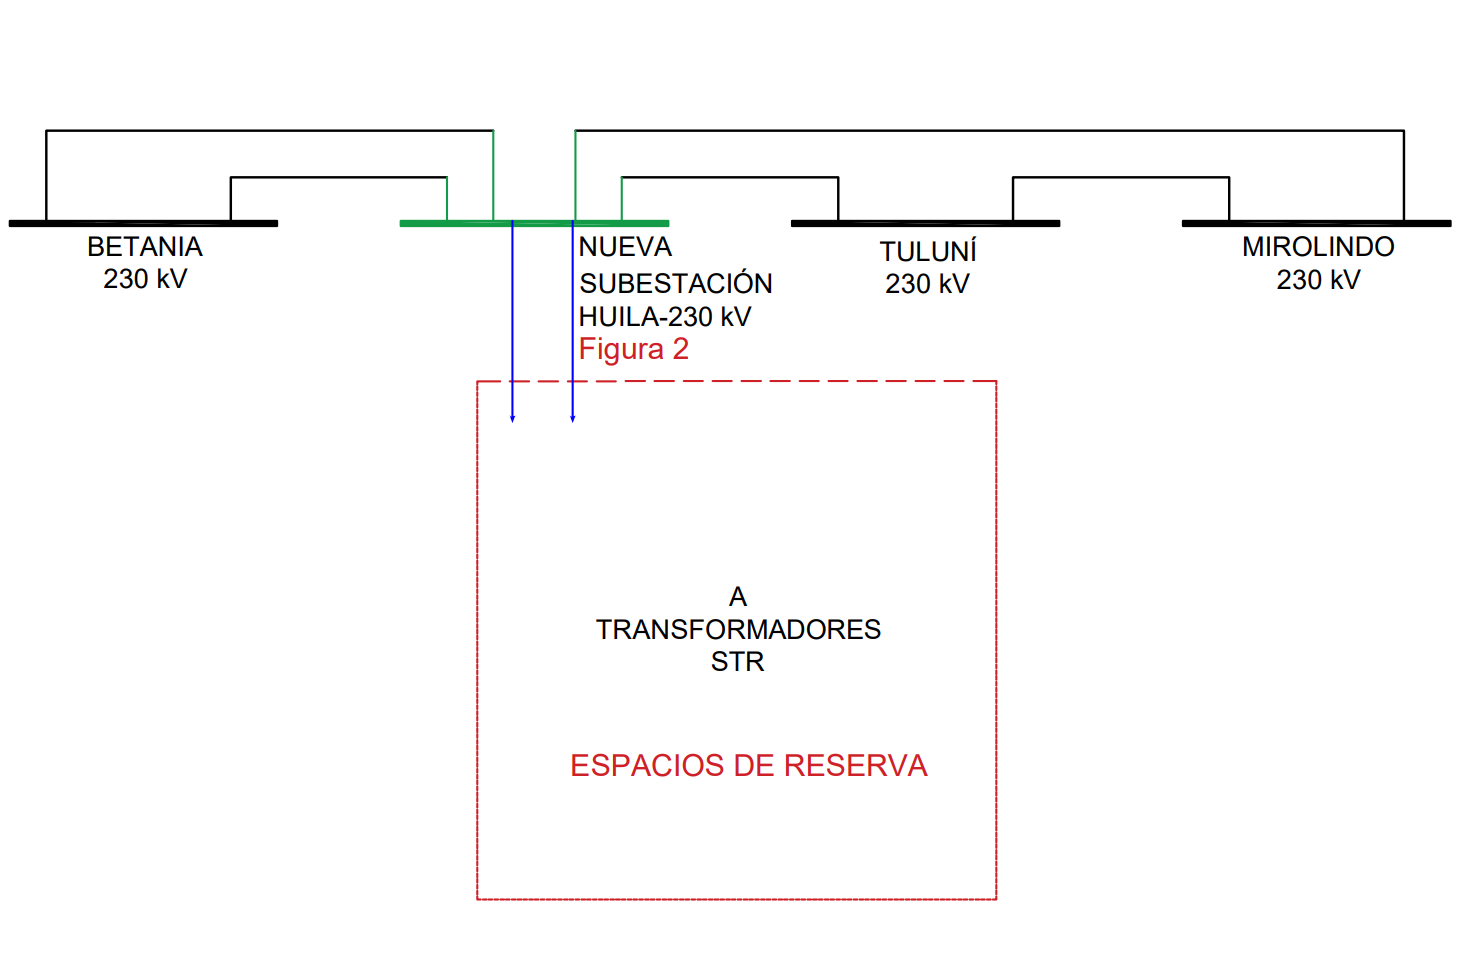
\includegraphics[width=1\textwidth]{1mer avance foticos/Esquema unifilar diagrama esquemático.png}
        \caption{en la figura del diagrama unifilar esquemático como\\ se evidenciará mas adelante en el trazado de la ruta se \\conectará la nueva subestación Huila de dicha forma.} % Título de la figura
        \label{fig:Esquema} % Etiqueta para referencias
    \end{subfigure}
    \hfill % Espacio horizontal entre las subfiguras
    \begin{subfigure}{0.5\textwidth}
        \centering % Centra la imagen
        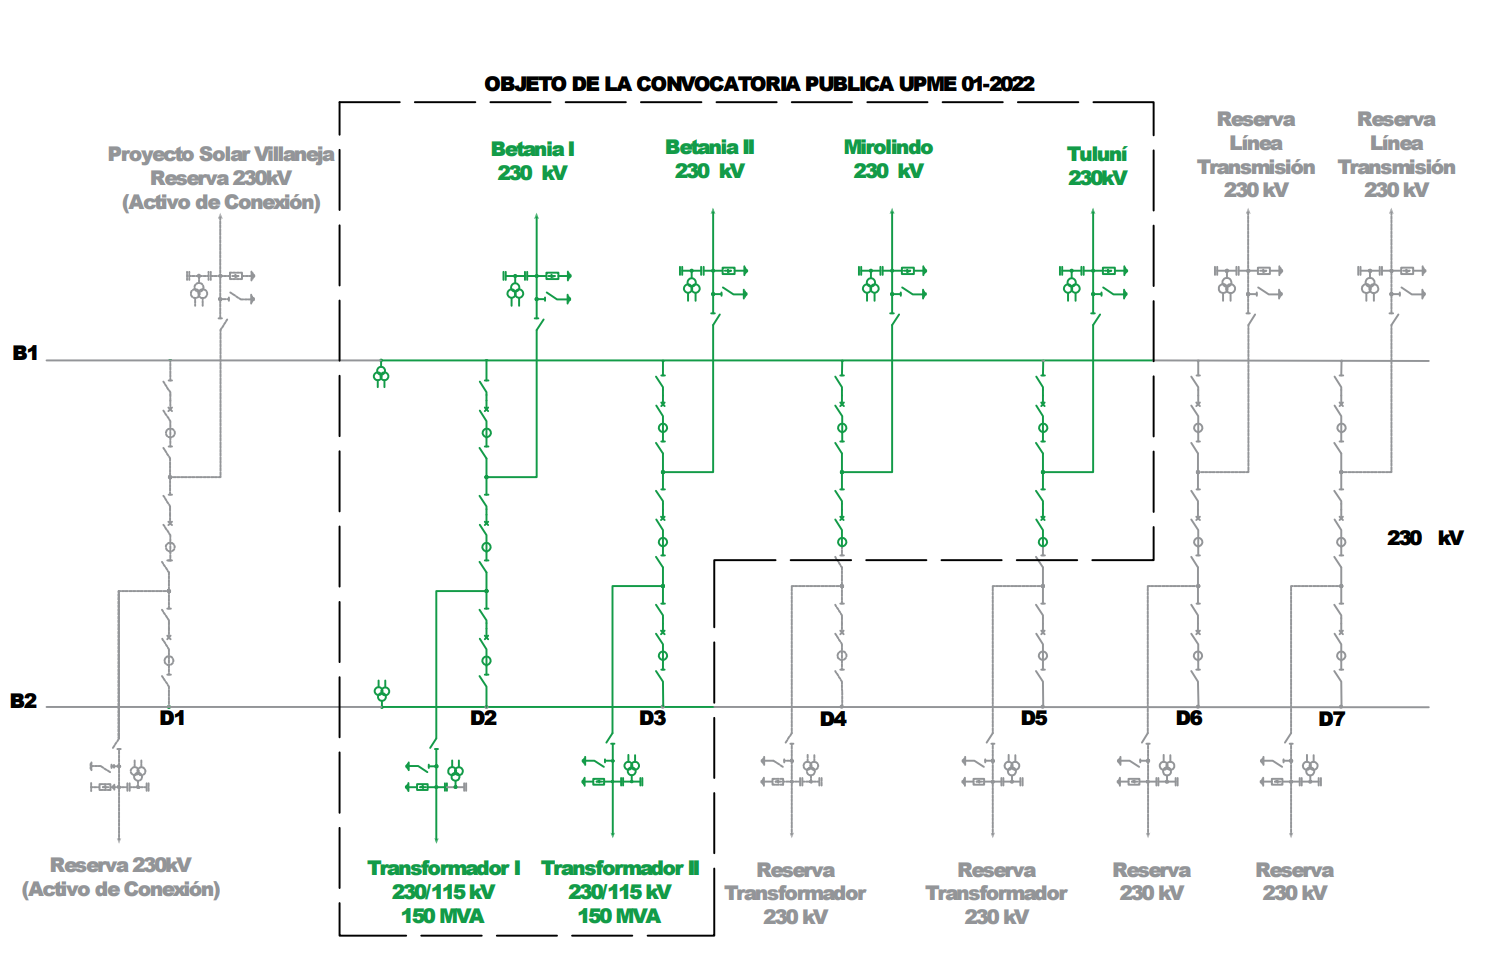
\includegraphics[width=1\textwidth]{1mer avance foticos/Esquema unifilar de la subestación huila 230kv.png}
        \caption{Esquema unifilar de la subestación huila 230kv.} % Título de la figura
        \label{fig:unifilar} % Etiqueta para referencias
    \end{subfigure}
    \label{fig:dos-imagenes}
\end{figure}



%En la \figurename~\ref{fig:unifilar} se muestra un ejemplo de cómo insertar y referenciar imágenes en LaTeX. Este formato permite que, si la imagen se mueve a otra parte del documento, la referencia se actualice automáticamente.



\section{Parámetros de Diseño Según la CREG025 – 1995}
\subsection{Frecuencia}
El valor nominal de la frecuencia del SIN colombiano es de 60,00 Hz.

\subsection{Tensión}
La tensión nominal del STN es de 220 kV y 500 kV. No obstante, para efectos de diseño de nuevas instalaciones, se exige una tensión nominal de 230 kV.

\subsection{Longitud de la Línea de Transmisión}
En todas las actividades relacionadas con diseño, cálculo, tendido, estimación de materiales y construcción, se entiende que la línea de transmisión está comprendida entre los pórticos de salida de cada subestación que sirve de fijación al vano que las une a la primera torre.

\subsection{Conductores por Fase}
\begin{itemize}
    \item Resistencias eléctricas, medida en W/km a 20 grados C, debe ser igual o menor a la determinada por la UPME.
    \item Niveles de campos eléctricos y magnéticos:
    \begin{itemize}
        \item A borde de servidumbre = 5 kV/m
        \item Campo magnético = 1 Gauss
        \item Cruces de carreteras 10 a 12 kV/m
    \end{itemize}
    \item Niveles máximos de radio interferencia:
    \begin{itemize}
        \item Zonas rurales: 22 dB a 80 m del eje de la línea a 1000 kHz
        \item Zonas Urbanas: 22 dB a 40 m del eje de la línea a 1000 kHz
    \end{itemize}
    \item Cable de guarda: Todas las líneas de transmisión del STN deberán tener cable de guarda. Este deberá soportar el impacto directo de las descargas eléctricas atmosféricas.
    \item Aislamiento: Se define mediante combinación de las distancias mínimas, todo esto para evitar sobretensiones por descargas atmosféricas, de frecuencia industrial, etc.
\end{itemize}

\subsection{Comportamiento Mecánico del Conductor de Fase y Cable de Guarda}
En cualquier condición, la tensión longitudinal máxima en el conductor o cable de guarda no deberá exceder el 50\% de su correspondiente tensión de rotura.

\subsection{Estructuras}
El cálculo de estas, depende mucho del tipo de estructura, ya sea de suspensión, de retención o de terminal. También se asocian a si estos están en una condición normal o anormal, incluyendo parámetros de viento, temperatura, rotura de los conductores o cables de guarda, etc.

\subsection{Cimentaciones}
Las cimentaciones deberán resistir todas las hipótesis de carga que se estipulen para cada uno de los tipos de estructura.

\subsection{Localización de Estructuras}
La localización de las estructuras deberá cumplir con ciertos requisitos para la seguridad sobre el terreno y obstáculos, entre estos se encuentran las carreteras principales, árboles, cercas, ferrocarriles, ríos navegables, embalses, entre otros.

\subsection{Cadenas de Aisladores y Herrajes}
Los aisladores deberán ser fabricados en porcelana, vidrio o poliméricos.

\subsection{Puesta a Tierra}
Este sistema de puesta a tierra debe estar en cada estructura y ser diseñado según las condiciones específicas de las líneas.

\subsection{Servidumbres}
El ancho de la faja de servidumbre requerida será establecido por el propietario de la línea, ajustado con base en los niveles de campo electromagnético y de radio interferencia.

\section{Trazado de la ruta}
Para el desarrollo del presente proyecto, se ha realizado el trazado preliminar de la línea de transmisión eléctrica asociada a la nueva subestación Huila 230 kV, utilizando la herramienta Google Earth. Esta plataforma permitió identificar de manera georreferenciada el punto exacto de ubicación de la subestación y definir visualmente el recorrido óptimo de la línea, considerando los criterios ya mencionados. \\
Apoyandonos de la herramienta de Google Earth.


    \begin{figure}[h!] % 'h' coloca la figura aquí
        \hfill % Espacio horizontal entre las subfiguras
        \begin{subfigure}{0.5\textwidth}
            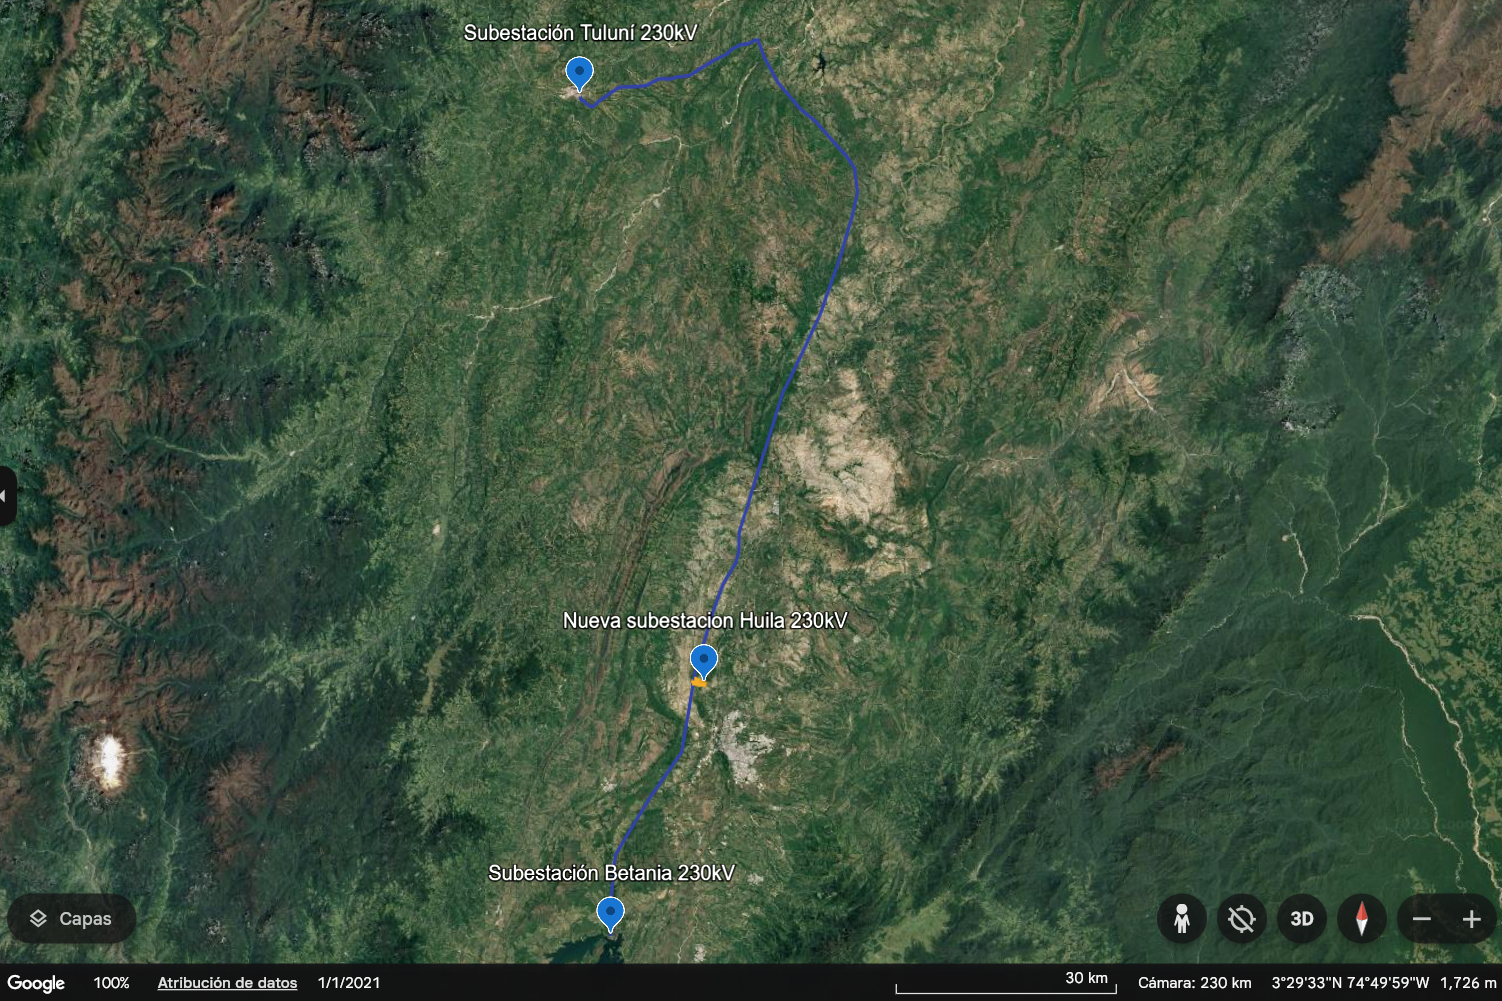
\includegraphics[width=1\textwidth]{1mer avance foticos/Huila 230kV - Google Earth - sin mirolindo.png}
            \caption{Nueva subestación huila conectada a la subestación Tuluní y Betania.} % Título de la figura
            \label{fig:sin mirolindo} % Etiqueta para referencias
        \end{subfigure}
        \begin{subfigure}{0.5\textwidth}
            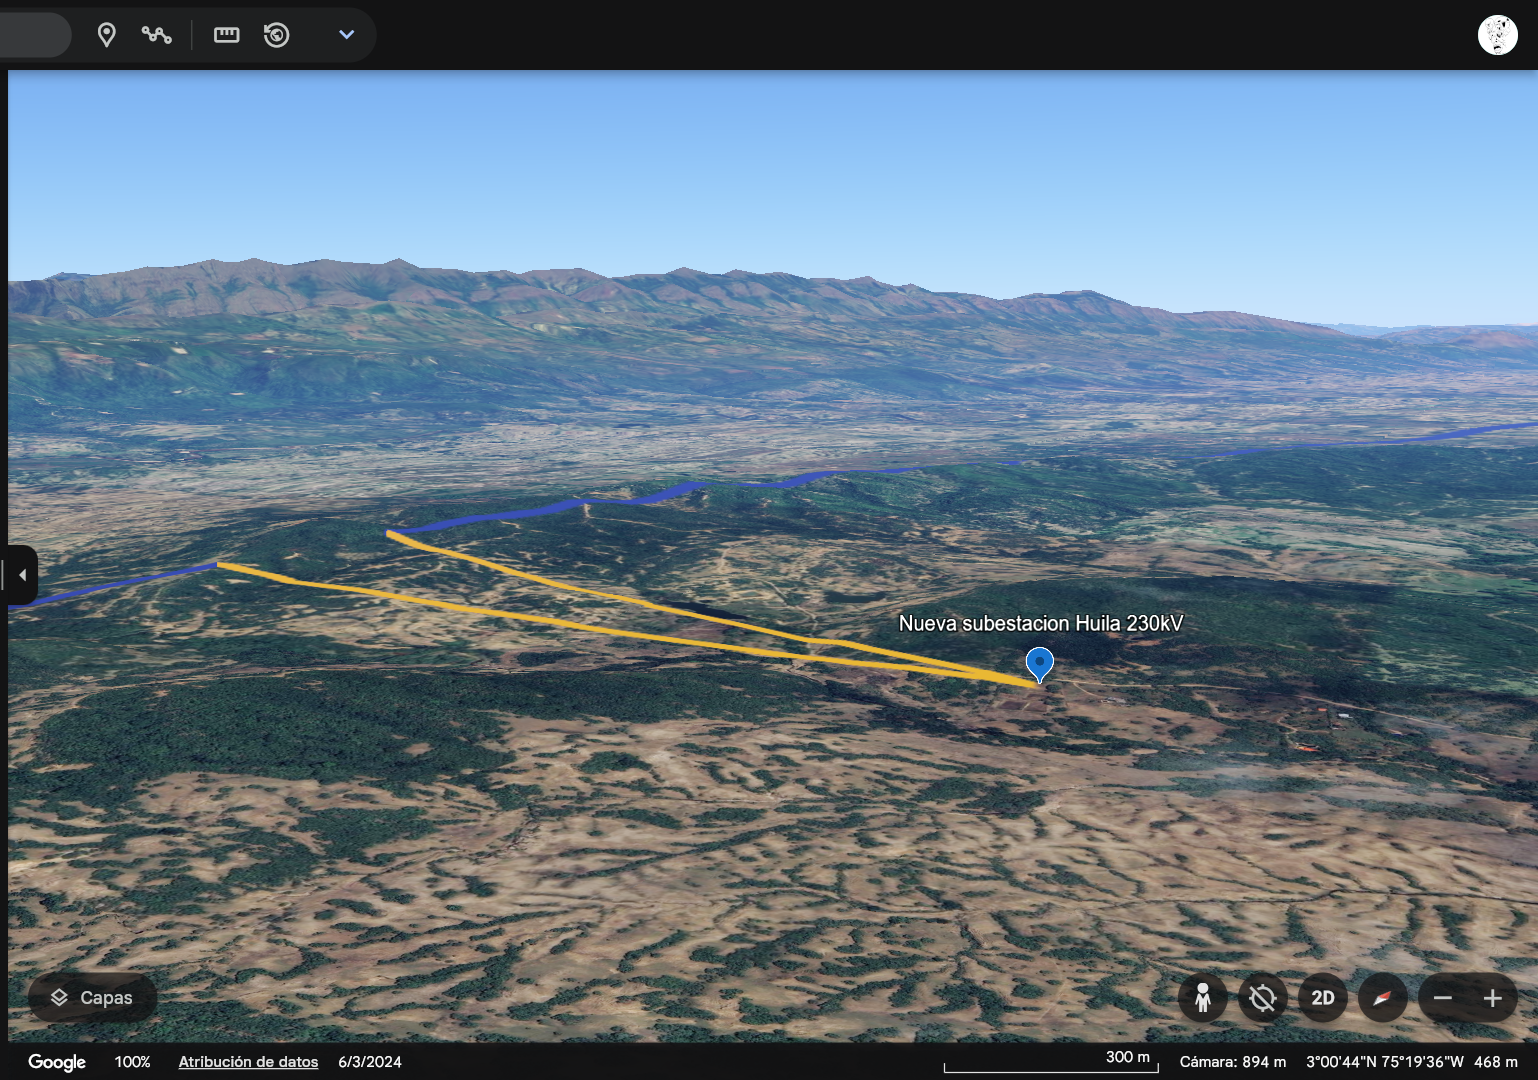
\includegraphics[width=1\textwidth]{1mer avance foticos/Huila 230kV - Google Earth - nueva acercada.png}
            \caption{Acercamiento a la nueva subestación huila conectada a la subestación Tuluní, Betania y Mirolindo.} % Título de la figura
            \label{fig:nueva acercada} % Etiqueta para referencias
        \end{subfigure}
    \end{figure}

    \begin{figure}[h!] % 'h' coloca la figura aquí
        \begin{subfigure}{0.5\textwidth}
            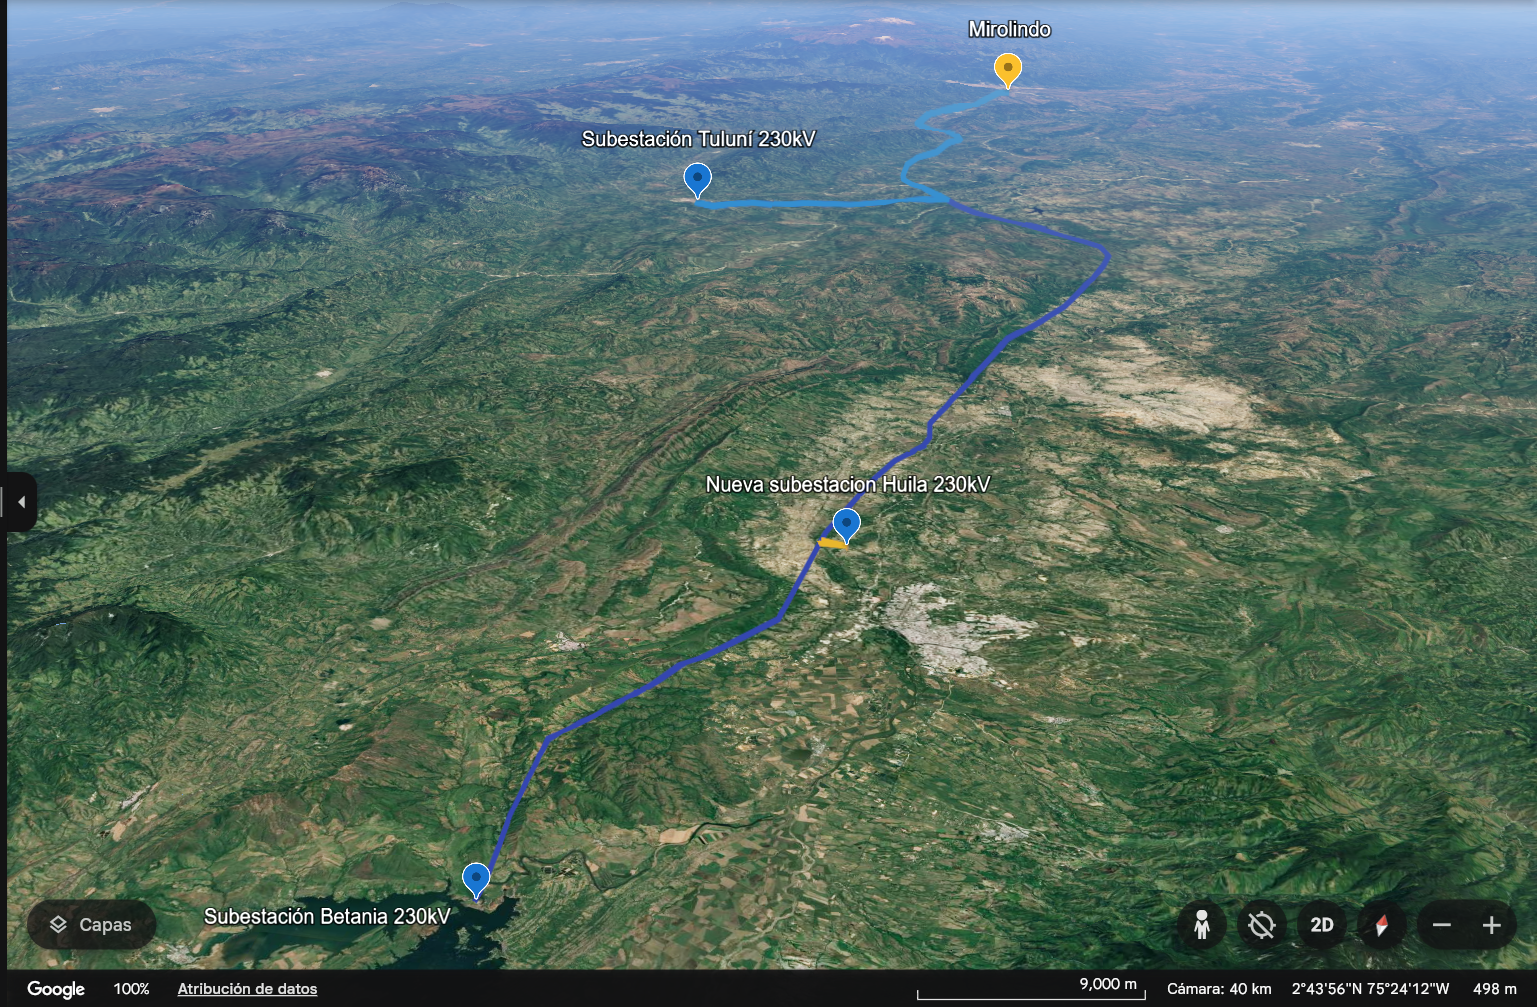
\includegraphics[width=1\textwidth]{1mer avance foticos/Huila 230kV - Google Earth - completo inclinado.png}
            \caption{Nueva subestación huila conectada a Betania con Mirolindo y conectada con Betania con Tuluní.} % Título de la figura
            \label{fig:todo angulo} % Etiqueta para referencias
        \end{subfigure}
        \hfill % Espacio horizontal entre las subfiguras
        \begin{subfigure}{0.5\textwidth}
            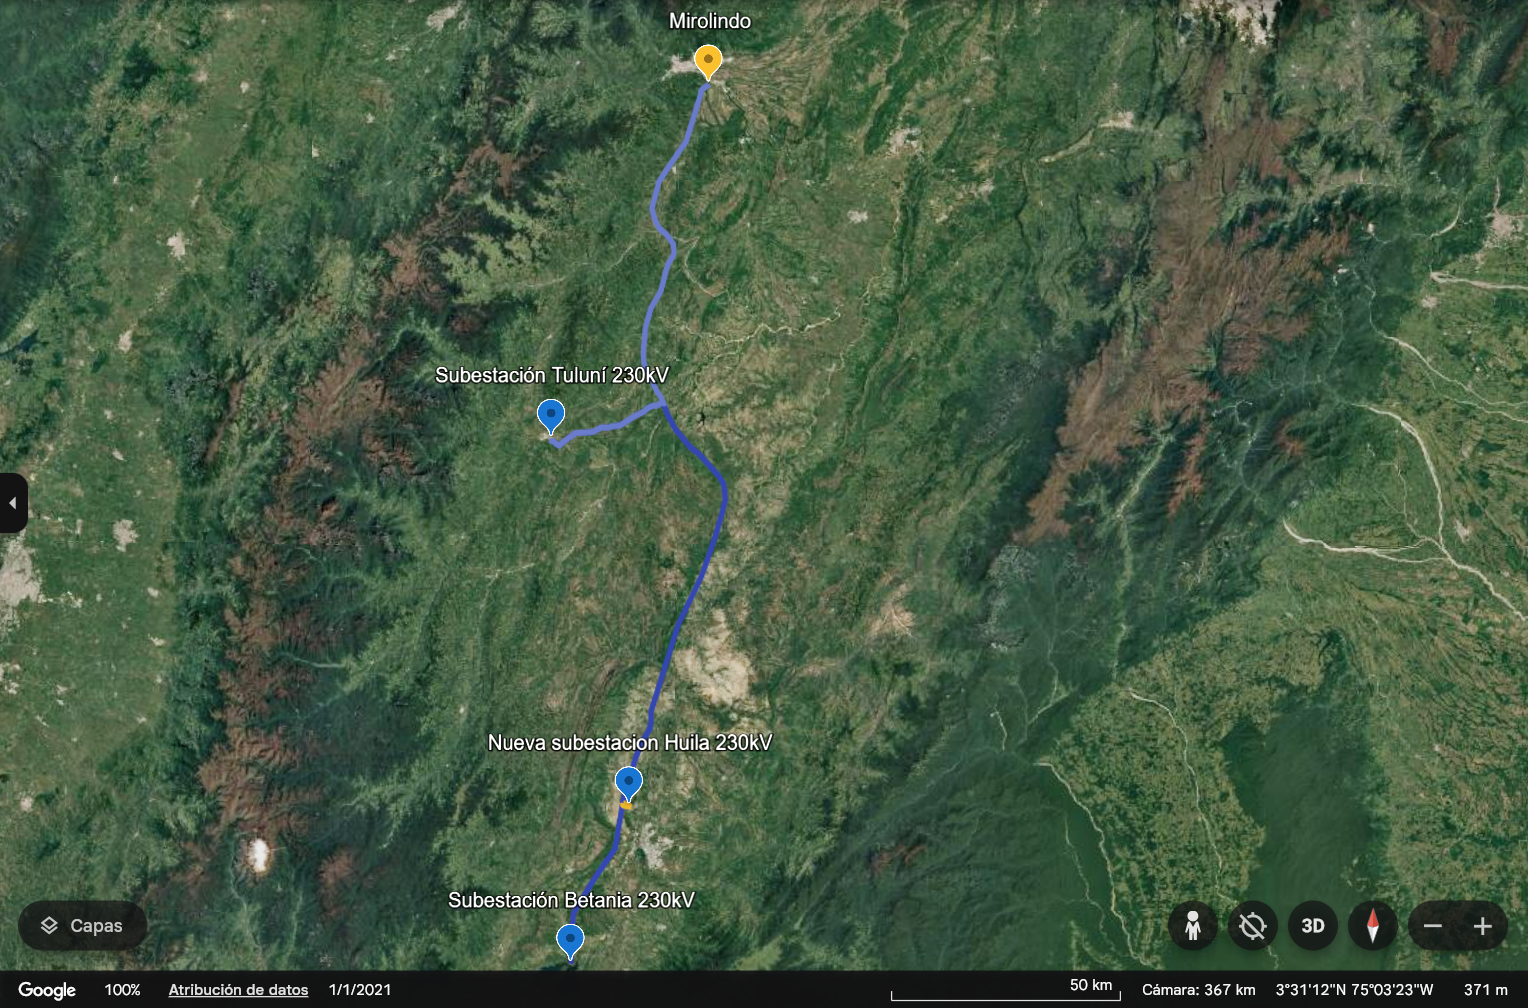
\includegraphics[width=1\textwidth]{1mer avance foticos/Huila 230kV - Google Earth - completo.png}
            \caption{Nueva subestación huila conectada a las lineas asociadas.} % Título de la figura
            \label{fig:todo} % Etiqueta para referencias
        \end{subfigure}
    \end{figure}

    \newpage


\section{Criterios para el trazado de la ruta}

\subsection{Criterios Socioeconómicos}
\begin{itemize}
    \item Población y Demografía
    \subitem Se consideran la distribución y densidad poblacional, así como la estructura de edad y género en las zonas de influencia. Estos datos permiten dimensionar la demanda de servicios, la disponibilidad de mano de obra y el posible impacto social.
    \\
    \item Tenencia de la Tierra y Restitución
    \subitem Se analiza la distribución de la propiedad, los tipos de tenencia (privada, colectiva, pública) y la existencia de procesos de restitución de tierras. Esto permite anticipar posibles conflictos de uso y definir estrategias para la gestión predial.
    \\
    \item Comunidades Étnicas y Actores Sociales
    \subitem Se identifican diferentes comunidades. El objetivo es garantizar la participación, el reconocimiento de sus derechos y la consideración de sus dinámicas culturales.
    \\
    \item Superposición con Otros Proyectos
    \subitem Se consideran iniciativas en curso o planificadas (infraestructura, hidrocarburos, minería, agricultura, etc.) para identificar sinergias y prevenir impactos acumulativos o conflictos en la ocupación del territorio.
\end{itemize}

\subsection{Criterios Físicos}
\begin{itemize}
    \item Estabilidad del Terreno
    \subitem Se evalúan las características geológicas y estructurales para determinar posibles deformaciones en la corteza y la historia geológica del área. Asimismo, se consideran amenazas naturales como la sismicidad y la remoción en masa (deslizamientos, derrumbes, etc.), que pueden afectar la infraestructura y la seguridad en la zona de influencia.
    \\
    \item Contaminación y Erosión
    \subitem Se identifican los factores que podrían generar deterioro en la calidad del aire, del suelo y de las fuentes hídricas. De igual manera, se revisan los procesos de erosión y sedimentación que pueden incrementarse con las actividades de construcción, buscando medidas de control y prevención.
    \\
    \item Recursos Hídricos
    \subitem Incluye la revisión de la disponibilidad y calidad del agua, tanto superficial como subterránea. Se procura salvaguardar los cuerpos de agua y sus zonas de protección, asegurando la sostenibilidad del recurso y minimizando posibles impactos en los ecosistemas asociados.
    \\
    \item Uso del Suelo y Paisaje
    \subitem Se analizan las vocaciones y usos actuales del suelo, así como los lineamientos de ordenamiento territorial. El objetivo es integrar la infraestructura de manera armónica con el entorno, reduciendo impactos visuales y protegiendo la calidad del paisaje local.
\end{itemize}
%Criterios rabon Dai
\subsection{Criterios de seguridad}
\begin{itemize}
    \item El trazado debe mantenerse alejado de áreas con amenaza de deslizamientos, inundaciones, fallas geológicas o incendios forestales, frecuentes en algunas zonas del Huila.
    
    \item La ruta debe permitir el acceso seguro para brigadas de mantenimiento y reparación sin exponer al personal a riesgos innecesarios.
    
    \item Las líneas de transmisión deben diseñarse y ubicarse considerando la protección con zonas habitadas, vías, cultivos, estructuras y el entorno, manteniendo distancias mínimas de seguridad que cumplan con las normativas eléctricas vigentes para minimizar riesgos de descargas, cortocircuitos o accidentes.
\end{itemize}

%falta añadir los criterios mios 
\section{IDENTIFICACIÓN DE LOS COMPONENTES DE UNA LÍNEA DE TRANSMISIÓN ELÉCTRICA EN EL ÁREA METROPOLITANA DE BUCARAMANGA}

La torre de transmisión analizada (\figurename~\ref{fig:Torre}) corresponde a la torre 002 de la subestación ESSA en Floridablanca, sede Ruitoque Bajo. Se trata de una torre de suspensión con doble circuito y tres fases. Una de las líneas pertenece al circuito Río Frío - Florida, mientras que la otra corresponde al circuito Conucos - Florida, los cuales alimentan distintas zonas del sistema eléctrico.

Los principales componentes son:

\begin{itemize}
    \item \textbf{$1.$ Circuito eléctrico:} La línea cuenta con un doble circuito.
    \item \textbf{$2.$ Conductores de fase:} Son los cables principales encargados de transportar la energía eléctrica a alta tensión. Se observan tres fases por circuito, cumpliendo con la configuración estándar.
    \item \textbf{$3.$ Aisladores:} Se identificaron cadenas de aisladores de suspensión, cuya función es separar eléctricamente los conductores de la estructura metálica de la torre, evitando cortocircuitos y pérdidas de energía.
    \item \textbf{$4.$ Cable de guarda con conexión a tierra:} Situado en la parte superior de la torre, protege la línea contra descargas atmosféricas (rayos) y disipa la corriente hacia tierra a través del sistema de puesta a tierra.
    \item \textbf{$5.$ Placa de identificación:} Contiene información sobre la línea, incluyendo el nombre del propietario y los datos técnicos relevantes.
    \item \textbf{$6.$ Dispositivo antiescalamiento:} Instalado en la base de la torre para evitar accesos no autorizados, contribuyendo a la seguridad del personal y de terceros.
    \item \textbf{$7.$ Amortiguador de vibraciones:} Se utiliza para reducir las vibraciones eólicas en los conductores de la línea de transmisión. Estas vibraciones son causadas por el viento, lo que puede generar fatiga en el cable y dañarlo con el tiempo.
    \item \textbf{$8.$ Puesta a tierra:} Su función principal es proteger la estructura y los equipos contra sobretensiones, especialmente descargas atmosféricas.
\end{itemize}



\begin{figure}[h!] % 'h' coloca la figura aquí
    \centering % Centra la imagen
    \begin{subfigure}{0.5\textwidth}
        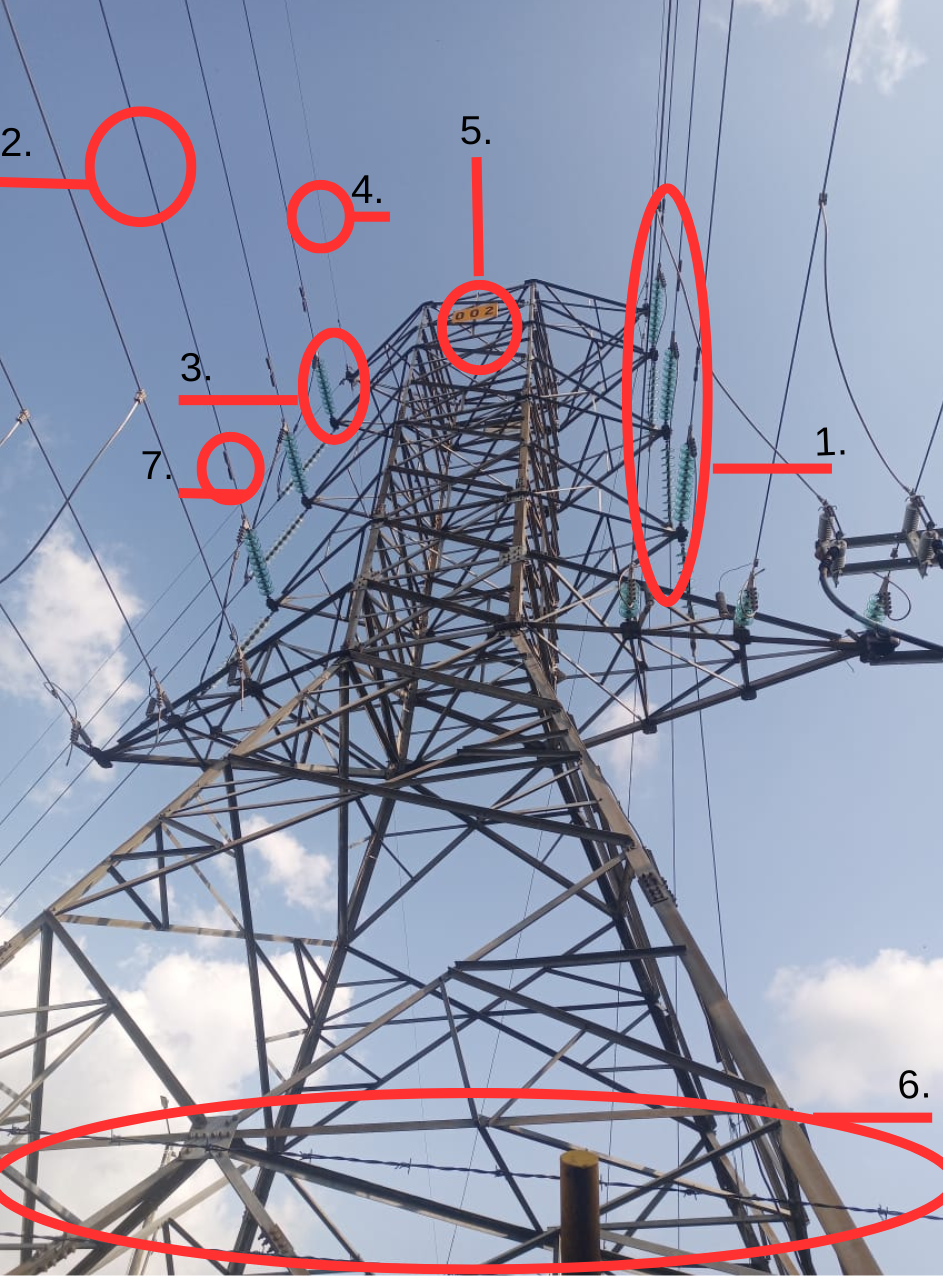
\includegraphics[width=1\textwidth]{1mer avance foticos/Torre.png}
        \caption{Torre 002 de la subestación ESSA en Floridablanca.} % Título de la figura
        \label{fig:Torre} % Etiqueta para referencias
    \end{subfigure}
    \hfill % Espacio horizontal entre las subfiguras
    \begin{subfigure}{0.5\textwidth}
        \centering % Centra la imagen
        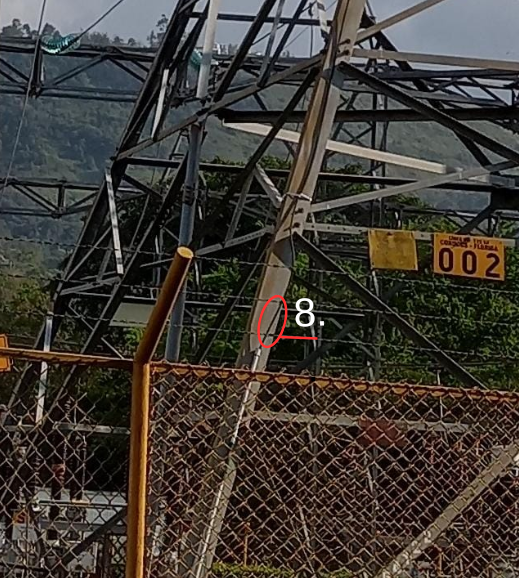
\includegraphics[width=1\textwidth]{1mer avance foticos/Torre-8.png}
        \caption{Cable de puesta a tierra de la torre 002 de la subestación ESSA en Floridablanca.} % Título de la figura
        \label{fig:Torre-8} % Etiqueta para referencias
    \end{subfigure}
\end{figure}


\section{Dimensiones y Distancias de Aislamiento}

Las principales dimensiones y distancias de aislamiento de la estructura son las siguientes:

\begin{itemize}
    \item Distancia mínima de servidumbre: 20 m.
    \item Distancia entre fases: Aproximadamente 2 m.
    \item Distancia al suelo: Aproximadamente 7 m, cumpliendo con los requisitos del RETIE.
    \item Longitud de las cadenas de aisladores: 2 m.
\end{itemize}

\section{Cumplimiento con el RETIE}

Basándonos en la observación y sin realizar mediciones directas, se pueden analizar algunos requisitos del Reglamento Técnico de Instalaciones Eléctricas (RETIE):

\begin{itemize}
    \item \textbf{Distancia de seguridad al suelo:} La separación observada parece cumplir con la normativa, que establece un mínimo de 7 metros en zonas de tránsito restringido.
    \item \textbf{Aisladores y distancias de seguridad:} La longitud de los aisladores y la separación entre fases parecen adecuadas para evitar descargas disruptivas.
    \item \textbf{Sistema de puesta a tierra:} La presencia del cable de guarda sugiere que la torre cuenta con un sistema de protección contra sobretensiones.
    \item \textbf{Identificación y seguridad:} La existencia de una placa de identificación y un dispositivo antiescalamiento indica que la estructura cumple con los requisitos de señalización y seguridad establecidos en el RETIE.
\end{itemize}

\section*{Conclusiones}
\begin{itemize}
    \item A partir del análisis comparativo realizado sobre los parámetros de diseño que establece la CREG 025 – 1995 y los descritos en la convocatoria de la UPME, se puede afirmar que cumplen con la normativa establecida en cuanto a la tensión, frecuencia, conductores, niveles de radiointerferencia, entre otros, garantizando de esta manera la confiabilidad de operación de nuestro sistema.\\
    \item Se concluye la importancia de tomar en cuenta los criterios socioeconómicos, los criterios físicos y los criterios de seguridad para la construcción y realización de la convocatoria, ya que por medio de estos se establecen las pautas requeridas, tales como minimizar los impactos en el medio ambiente y comunidades cercanas, así como las evaluaciones del terreno y el entorno para garantizar la confiabilidad del proyecto, entre otros.\\
    \item Con base en los requisitos del Reglamento Técnico de Instalaciones Eléctricas (RETIE) y a través de la observación directa de la salida de campo, donde se evidenciaron los principales componentes de la torre de transmisión, así como también el dimensionamiento y distancias de la misma, se concluye que esta cumple con los requisitos mínimos de distancias de seguridad, aisladores y puesta a tierra que se establecen.
\end{itemize}



\end{document}  
